% SIPAIM 2026 -- TEM Axon & Myelin Segmentation Challenge: method description.
% SIPAIM template (IEEEtran, journal option). Max. 4 pages + 1 page of references.
% Numbers marked with the macros below are filled from the evaluation scripts.

\documentclass[journal]{IEEEtran}
\IEEEoverridecommandlockouts

\usepackage{cite}
\usepackage{graphicx}
\usepackage{amsmath,amssymb}
\usepackage{booktabs}
\usepackage{url}

\def\BibTeX{{\rm B\kern-.05em{\sc i\kern-.025em b}\kern-.08em
    T\kern-.1667em\lower.7ex\hbox{E}\kern-.125emX}}


\begin{document}

\title{Geometric-Prior nnU-Net for Paired Axon and Myelin Instance Segmentation in Transmission Electron Microscopy}

% TODO (authors): complete surnames, affiliation and contact e-mail.
\author{%
    \IEEEauthorblockN{Danitza Bermejo\textsuperscript{*},
    Gabriel Omar Dur\'an Ruiz\textsuperscript{*},
    Valeria \textless Surname\textgreater,
    Dhiago \textless Surname\textgreater}
    \\
    \IEEEauthorblockA{\textit{\textless Department\textgreater, \textless Institution\textgreater, \textless City\textgreater, \textless Country\textgreater}}\\
    \IEEEauthorblockA{\textless corresponding e-mail\textgreater \quad \textsuperscript{*}Equal contribution}
}

\maketitle

\begin{abstract}
Per-fiber g-ratio measurement in transmission electron microscopy requires
every axon to be segmented as an instance paired with its own myelin sheath.
We present GPEM15, a two-dimensional nnU-Net that receives a fixed,
twelve-channel geometric prior describing the core, ring and surround
structure of myelinated fibers. The prior enters the three deepest encoder
stages through zero-initialized learned gates, so training starts from a plain
nnU-Net and the network decides how much geometry to use. Training adds a
g-ratio consistency term, an edge-band term on the myelin boundary and an
auxiliary per-fiber acceptance head. Instances are assembled by watershed from
the predicted axons; fibers whose myelin covers less than half of the ring
around the axon and fibers cut by the image border are removed. On the 54
validation images of the first fold, GPEM15 reaches a mean
Dice of 0.884, an HD95 of 583~nm and a g-ratio mean absolute error of
0.0133, against 0.853, 608~nm and 0.0157 for a fine-tuned two-model
Cellpose-SAM pipeline evaluated out of fold on the same images.
\end{abstract}

\begin{IEEEkeywords}
transmission electron microscopy, axon, myelin, g-ratio, instance segmentation, nnU-Net, Cellpose-SAM
\end{IEEEkeywords}

% =====================================================================
\section{Introduction}

Quantitative morphometry of myelinated axons is central to the study of
demyelinating and neurodegenerative disease. Its main biomarker, the g-ratio
$g = D_{\text{axon}}/D_{\text{fiber}}$~\cite{chomiak2009}, must be measured per
fiber, so each axon has to be delineated as an instance and linked to its own
myelin sheath. AxonDeepSeg~\cite{zaimi2018} and the self-configuring
nnU-Net~\cite{isensee2021} segment axon and myelin semantically and recover
instances in post-processing, whereas Cellpose~\cite{stringer2021} and
Cellpose-SAM~\cite{pachitariu2025} predict instances directly.

In the challenge images, a myelinated fiber appears as a light axoplasm
enclosed by a thin dark myelin ring. Our design hypothesis is that an explicit
description of this core--ring--surround layout, measured at several radii,
helps the network separate fibers from other structures with similar local
texture. Our contributions are: (i) a fixed geometric prior fused
into nnU-Net through learned gates that start closed; (ii) training terms
tailored to the challenge metrics (g-ratio and myelin boundary); and (iii) an
objective comparison, on identical images and with the official metrics,
against a strong instance-native alternative based on Cellpose-SAM.

% =====================================================================
\section{Data and Evaluation}

The challenge provides 266 annotated TEM images of the mouse corpus callosum
($3008\times4096$ pixels, 2.152~nm/pixel) with 16-bit paired instance labels:
0 background, 1 artifact (ignored), even $X\geq2$ axon and $X+1$ its myelin.
The metrics are the Dice similarity coefficient (DSC) of the axon (even labels)
and myelin (odd labels $\geq3$) compartments; the 95th-percentile Hausdorff
distance (HD95), the larger of the two directed 95th percentiles of
boundary distances, in nm; and the mean absolute error of the per-fiber
g-ratio (MAE$_g$), with $D=2\sqrt{A/\pi}$, over predicted fibers matched to
reference fibers by IoU. We implemented these definitions and report DSC and
HD95 averaged over images (mean of both compartments) and MAE$_g$ pooled over
matched fibers. GPEM15 uses the default nnU-Net 5-fold split (54/53/53/53/53
images); Cellpose-SAM was cross-validated with its own random 5-fold split.

% =====================================================================
\section{Method}

\begin{figure*}[t]
\centering
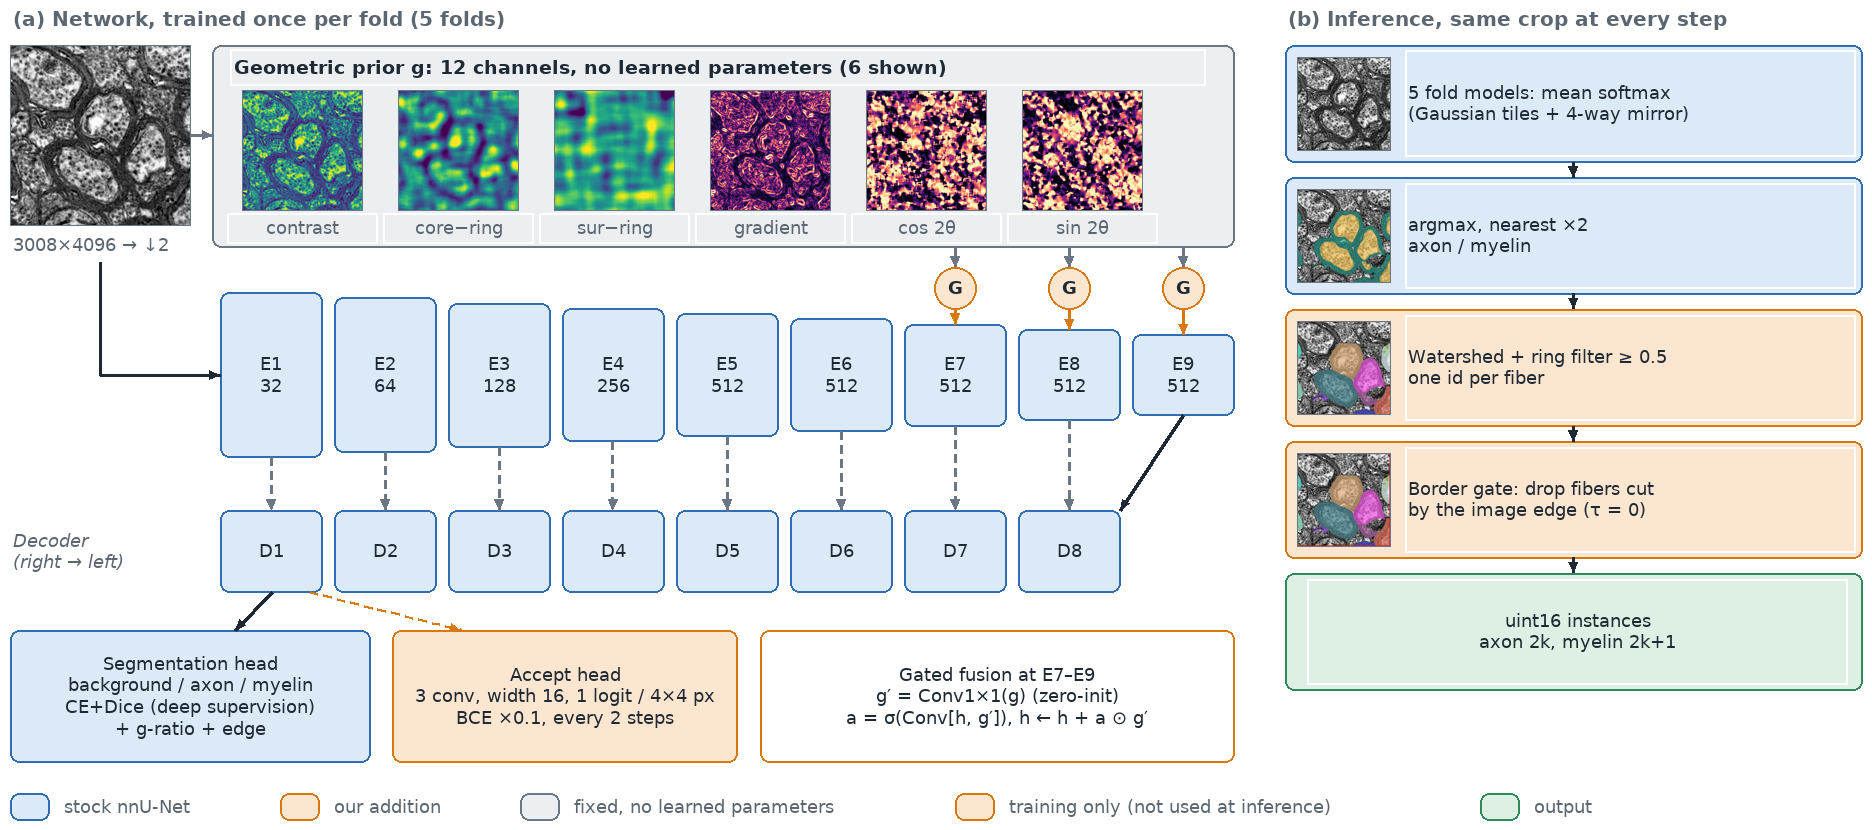
\includegraphics[width=\textwidth]{figures/gpem15_method.png}
\caption{GPEM15. (a) A 12-channel geometric prior $g$, computed from the image
without learned parameters, enters the last three encoder stages of a 9-stage
2D nnU-Net through learned per-pixel gates. During training only, an accept
head predicts a per-fiber score. (b) Inference: softmax of the fold models,
watershed instance assembly, ring filter and border gate.}
\label{fig:method}
\end{figure*}

\subsection{Network}
GPEM15 is the 2D configuration of nnU-Net~\cite{isensee2021} (plain
convolutional encoder--decoder with 9 stages of 32--512 channels, patch
$1024\times1536$, batch size 2, as planned by nnU-Net for the training images
downsampled by 2) with three classes, background, axon and myelin; artifact
pixels are an ignore label.

\subsection{Geometric prior and gated fusion}
From the input image we compute, with square box filters on its integral
image, twelve maps: a local contrast map (the image minus a large box mean);
for each radius $r\in\{20,30,45,68\}$ pixels, the mean intensity of a core
window (half-size $0.6r$) minus that of a ring window ($0.9r$--$1.4r$), and of
a surround window ($1.6r$--$2.2r$) minus the ring; the gradient magnitude of the
smoothed image; and the local orientation $(\cos2\theta,\sin2\theta)$ from
the structure tensor (Fig.~\ref{fig:method}a). The core--ring and
surround--ring maps are designed to respond to a light region enclosed by a
darker ring of radius about $r$. The prior has no learned parameters. At each of the three deepest encoder stages, with features
$h$, it is resized, projected by a $1\times1$ convolution $P$ initialized to
zero, and added through a gate:
\begin{equation}
h \leftarrow h + \sigma\!\left(G([h, Pg])\right)\odot Pg,
\end{equation}
where $G$ is a two-layer $1\times1$ convolutional network and the prior is
resized bilinearly to each stage. Because $P$ starts at zero, the network is
initially identical to nnU-Net.

\subsection{Training objective}
The loss is the nnU-Net cross-entropy plus Dice loss with deep supervision,
plus three terms. A g-ratio term penalizes
$|g_{\text{pred}}-g_{\text{true}}|$ per patch, with
$g=\sqrt{A_{\text{axon}}/(A_{\text{axon}}+A_{\text{myelin}})}$ computed from
soft areas. An edge term adds the cross-entropy restricted to a $7\times7$
band around the reference myelin boundary, where HD95 is measured. An accept
head (three convolutions on the last decoder features and the axon/myelin
probabilities) is trained with a balanced binary cross-entropy (weight 0.1,
every second iteration). Its targets are derived from the reference: a
predicted axon component is positive if it overlaps a reference axon with IoU
$\geq0.3$, and negative if it does not and its myelin ring is broken (at least
4 of 24 angular sectors with less than 30\% myelin); other components are
ignored. Each fold is trained for 150 epochs with bfloat16 mixed precision;
batches with non-finite loss or gradients are skipped.

\begin{table*}[t]
\caption{Validation on the 54 images of fold 0. Both methods are evaluated with
the same implementation of the challenge metrics; Cellpose-SAM predictions are
out of fold. Detected: reference fibers matched with IoU $\geq0.5$. Open:
predicted fibers (not touching the border) whose myelin does not enclose the
axon (reference annotations over the 266 images: 0.6\%).}
\label{tab:results}
\centering
\footnotesize
\setlength{\tabcolsep}{4pt}
\begin{tabular}{@{}lccccccccc@{}}
\toprule
 & \multicolumn{3}{c}{DSC $\uparrow$} & \multicolumn{3}{c}{HD95 (nm) $\downarrow$} & & & \\
\cmidrule(lr){2-4}\cmidrule(lr){5-7}
Method & axon & myelin & mean & axon & myelin & mean & MAE$_g$ $\downarrow$ & Detected $\uparrow$ & Open $\downarrow$ \\
\midrule
Cellpose-SAM (out of fold)            & 0.877 & 0.829 & 0.853 & 608 & 608 & 608 & 0.0157 & 96.0\% & \textbf{3.0\%} \\
GPEM15, full-resolution input         & 0.831 & 0.804 & 0.818 & 816 & 736 & 776 & 0.0219 & 91.3\% & 13.9\% \\
\textbf{GPEM15 (fold 0 model)}  & 0.893 & 0.876 & \textbf{0.884} & 608 & 559 & \textbf{583} & \textbf{0.0133} & 96.6\% & 4.2\% \\
\bottomrule
\end{tabular}
\end{table*}

\subsection{Instance assembly}
Inference uses the nnU-Net predictor (Gaussian-weighted sliding window with
mirroring; with several folds, their softmax outputs are averaged) and takes
the argmax. Each image is downsampled by 2 (2$\times$2 mean) before inference,
as in training, and the class map is brought back to full resolution by
nearest-neighbor upsampling; for the test set, the five fold models are
ensembled. Axon instances are the connected components of the axon class; the myelin is
assigned to axons by a watershed on the distance to the axons, restricted to
the foreground. Each axon $k$ and its sheath receive labels $2k$ and $2k+1$.
Fibers whose myelin covers less than half of a 4-pixel ring around the axon are
removed, as are fibers whose axon touches the image border, whose anatomy is
cut. The accept score is not used to filter fibers at inference
(Fig.~\ref{fig:method}b).

\subsection{Comparison method: Cellpose-SAM}
Two Cellpose-SAM models~\cite{pachitariu2025} are fine-tuned at scale 0.25 on
whole fibers and on axons (first 12 of 24 ViT blocks frozen, AdamW~\cite{loshchilov2019},
learning rate $10^{-5}$, up to 200 epochs with early stopping on validation
Dice); the myelin is the fiber minus its axon, so the pairing is valid by
construction. Inference lowers the cell-probability threshold to $-1$ and adds
a second pass at half scale. It was evaluated with its own 5-fold
cross-validation on the 266 images; its out-of-fold predictions on the 54
images of nnU-Net fold 0 are used below.

% =====================================================================
\section{Results}


Table~\ref{tab:results} compares both methods on the same 54 images. GPEM15
obtains the best DSC, HD95 and MAE$_g$, i.e., the best rank on the three
challenge criteria, and detects slightly more reference fibers; Cellpose-SAM
produces fewer open fibers, since its myelin is the fiber minus the axon.
Running GPEM15 on full-resolution images, i.e., at twice the scale seen in
training, degrades every metric (second row), so inference must use the
training resolution. Over its full 5-fold cross-validation
(266 images), Cellpose-SAM reaches a DSC of $0.862\pm0.014$, an HD95 of
$530\pm81$~nm and an MAE$_g$ of 0.0160 (mean $\pm$ standard deviation across
folds); its default inference gives 0.855, 563~nm and 0.0180.

In development experiments on fold 0 with earlier versions of the model, the
border gate lowered the HD95 from 721 to 575~nm, 150 training epochs gave a
lower HD95 than 20 or 250 epochs (591, 654 and 635~nm), and learned filters on
top of the per-fiber score raised its AUC without lowering the HD95.

% =====================================================================
\section{Discussion and Conclusion}

An explicit description of fiber geometry and metric-specific training terms
fit into nnU-Net without changing its architecture, and the zero-initialized
gates make training start from the plain network. On identical images,
GPEM15 scores better than an instance-native Cellpose-SAM pipeline on all
three challenge metrics, whereas Cellpose-SAM leaves fewer open myelin sheaths.
Limitations are that the post-processing and the number of epochs were chosen on
fold 0, which is also the fold reported in Table~\ref{tab:results}, that only
one fold of GPEM15 was evaluated, and that fibers touching the border are
discarded by design. The code and the five fold
models are provided with the submission.

\section*{Acknowledgment}
We thank the organizers of the TEM Axon \& Myelin Segmentation Challenge and the
Paris Brain Institute (ICM) for the annotated dataset.

\textit{Use of generative AI.} In accordance with the IEEE policy on
AI-generated content, we disclose that Claude (Anthropic; Claude Opus 5.5,
used through the Claude Code assistant) was used (i) to write and debug the
code of the Cellpose-SAM pipeline (training, early stopping, 5-fold
cross-validation, inference and evaluation scripts), the correction of the
input resolution in the GPEM15 inference script, the evaluation of both
methods with the challenge metrics and the comparison analyses reported in
Section~IV and Table~\ref{tab:results}; and (ii) to draft the text of this
manuscript from the authors' code, results and notes. % TODO (authors): add any AI use in the nnU-Net/GPEM15 code or in Fig. 1, or confirm there was none.
All AI-generated code and text were reviewed, verified against the
experimental outputs and edited by the authors, who take full responsibility
for the content of this paper.

\bibliographystyle{IEEEtran}
\bibliography{refs}

\end{document}
